%-------------------------------------------------------------------------------
%                                PREAMBLE
%-------------------------------------------------------------------------------
\documentclass[usenames,dvipsnames,svgnames,10pt,aspectratio=169]{beamer}
\usefonttheme{professionalfonts}

% This theme uses TIKZ: compile twice with PDFLaTeX or LuaLaTeX.
%
%  Options:
%  - [clean]:    clean slides, i.e. logos and footbar are removed
%  - [kth]:      footbar style inspierd to the official KTH template
%  - [nicewave]: a different style of wave is used (not approved by FLOW)
%
\usetheme{flow}

\usepackage{hyperref,graphicx,lmodern}
\usepackage[utf8]{inputenc}
\usepackage{media9}
\usepackage{xcolor}
\usepackage{stmaryrd}
\usepackage{nicefrac}
\usepackage{multimedia}
\usepackage{multicol}
\usepackage{upgreek}
\usepackage[]{bm}
\usepackage[]{url}

\DeclareMathOperator{\sinc}{sinc}
\DeclareMathAlphabet{\mathcal}{OMS}{cmsy}{m}{n}
\DeclareMathAlphabet\mathbfcal{OMS}{cmsy}{b}{n}

\graphicspath{{imgs/}}
\setbeamertemplate{blocks}[rounded][shadow=true]

\DeclareMathOperator{\trace}{tr}

%-------------------------------------------------------------------------------
%                                TITLE PAGE
%-------------------------------------------------------------------------------
\title[Nonlinear Physics] % Short title used in footline
{
	Nonlinear physics, dynamical \\ systems and chaos theory
}

\author[J.-Ch.~Loiseau] % Presenting author in short form used in footline
{
	Jean-Christophe Loiseau
}
% - Give the names in the same order as the appear in the paper.
% - Underline the presenting author.

\institute[unused]
{
	\url{jean-christophe.loiseau@ensam.eu} \\
	DynFluid, \\
	Arts et M\'etiers ParisTech, France
}
% Keep it simple, no one is interested in your street address.

% University logo(s)
\logot{
\includegraphics[width=.128\paperwidth]{DynFluid_logo}}  % Top logo
\logob{
\includegraphics[width=0.128\paperwidth]{ENSAM_logo}} % Bottom logo
% \logoc[{
\includegraphics[width=.128\paperwidth]{limsi}}]{
\includegraphics[width=.128\paperwidth]{limsi}} % Corner logo
%
% Cover image: \cvrimg{x position}{y position}{cover image}
\cvrimg{.77}{.8}{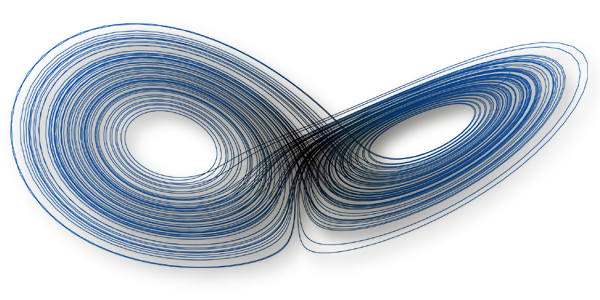
\includegraphics[width=.4\paperwidth]{cover.png}}

\date[unused]{ENSAM, Master 2, 2017--2018}

\begin{document}

\titleframe % Print the title as the first slide

%-------------------------------------------------------------------------------
%                           FLUIDIC PINBALL
%-------------------------------------------------------------------------------


\begin{frame}[t, c]{}
	\centering
	\vspace{1cm}

	{\Large \textbf{Fluidic pinball}}

	\bigskip

	{\textgre{\textbf{Platform for MIMO nonlinear flow control}}}

\end{frame}

\begin{frame}[t, c]{Fluidic Pinball}{Flow configuration}
	\begin{minipage}{.48\textwidth}
		\centering
		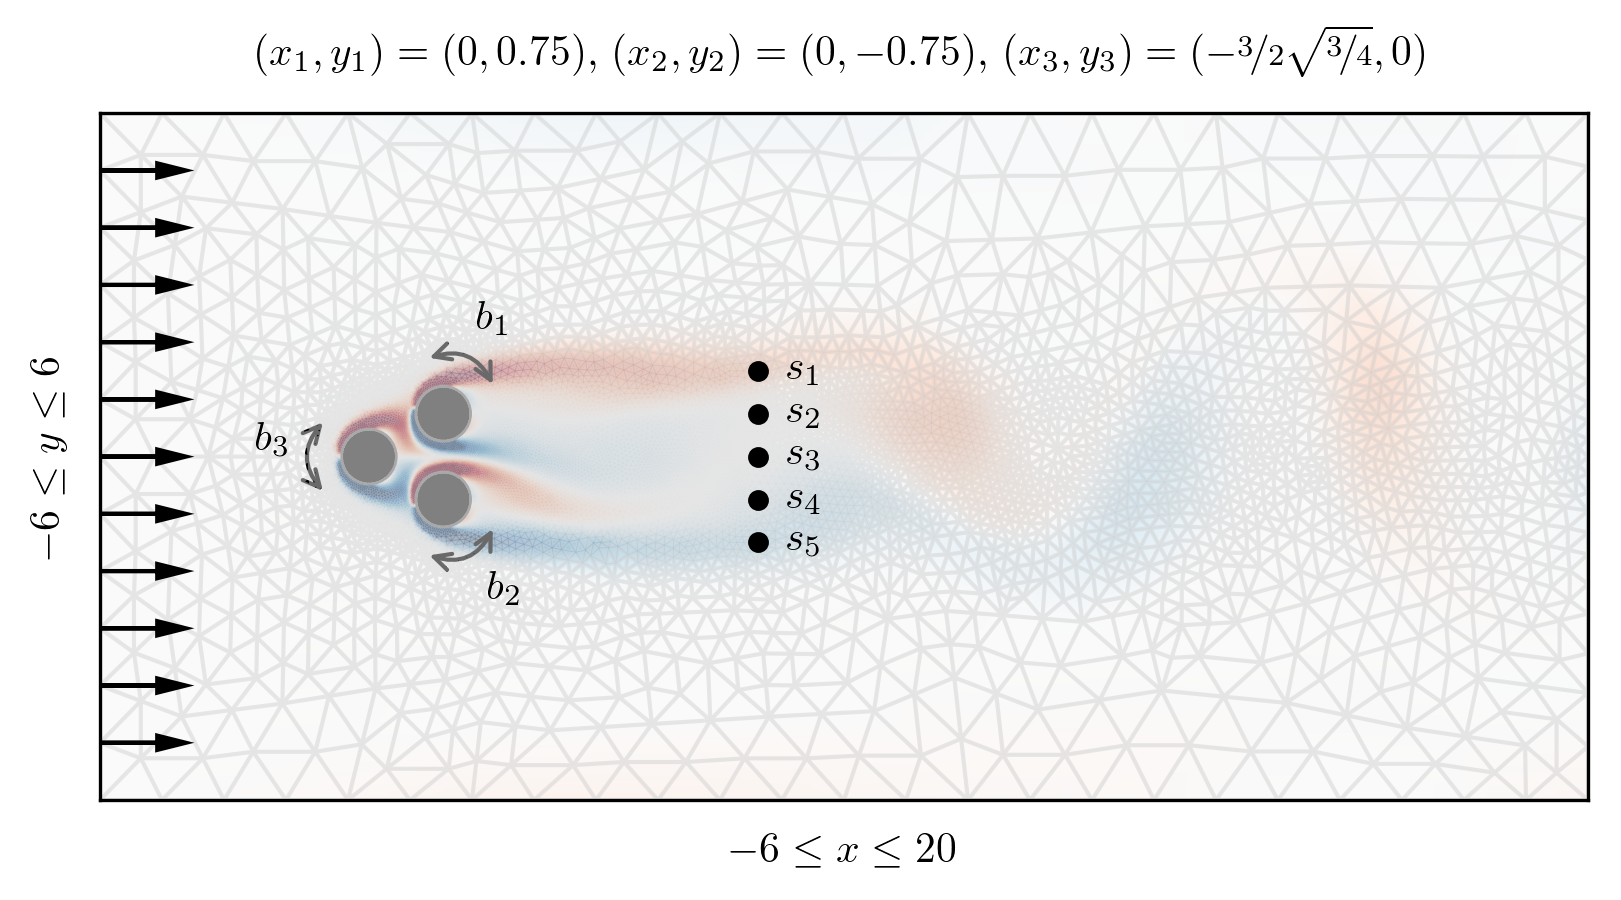
\includegraphics[width=.95\textwidth]{pinball_geometry}

		Geometry of the \emph{Fluidic pinball}.
	\end{minipage}%
	\hfill
	\begin{minipage}{.48\textwidth}
		\begin{itemize}
			\item New benchmark for nonlinear MIMO control mimicking experimental conditions.
			\begin{itemize}
				\item[$\hookrightarrow$] Five velocity sensors + lift forces.
				\item[$\hookrightarrow$] Control knobs: rotation of the cylinders.
				\item[$\hookrightarrow$] PIV-like vorticity snapshots.
			\end{itemize}

			\item DNS code by Marek Morzynski.
			\begin{itemize}
				\item[$\hookrightarrow$] 3\textsuperscript{rd} order accurate FEM.
				\item[$\hookrightarrow$] $\simeq 30$ minutes to simulate 100 convective time units.
			\end{itemize}

			\item Companion experiment at University of Calgary, Canada.
		\end{itemize}
	\end{minipage}

	\vspace{1cm}
\end{frame}

\begin{frame}[t, c]{Fluidic Pinball}{Overview of the dynamics}
	\begin{minipage}{.48\textwidth}
		\centering
		\movie[width=\textwidth, autostart, loop]{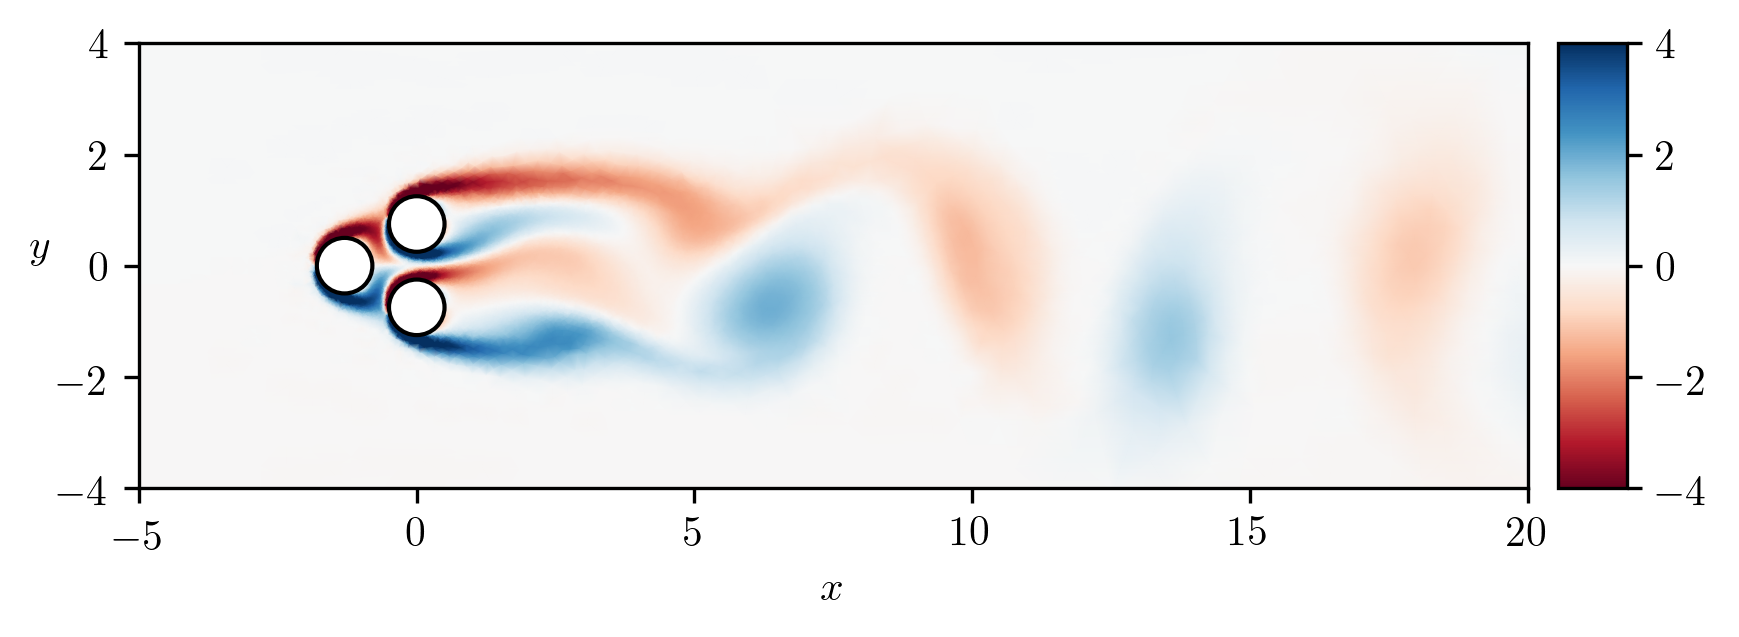
\includegraphics[width=\textwidth]{pinball_dynamics_Re100}}{imgs/pinball_dynamics_Re100.mp4}

		$Re = 100$
	\end{minipage}%
	\hfill
	\begin{minipage}{.48\textwidth}
		\centering
			\movie[width=\textwidth, autostart, loop]{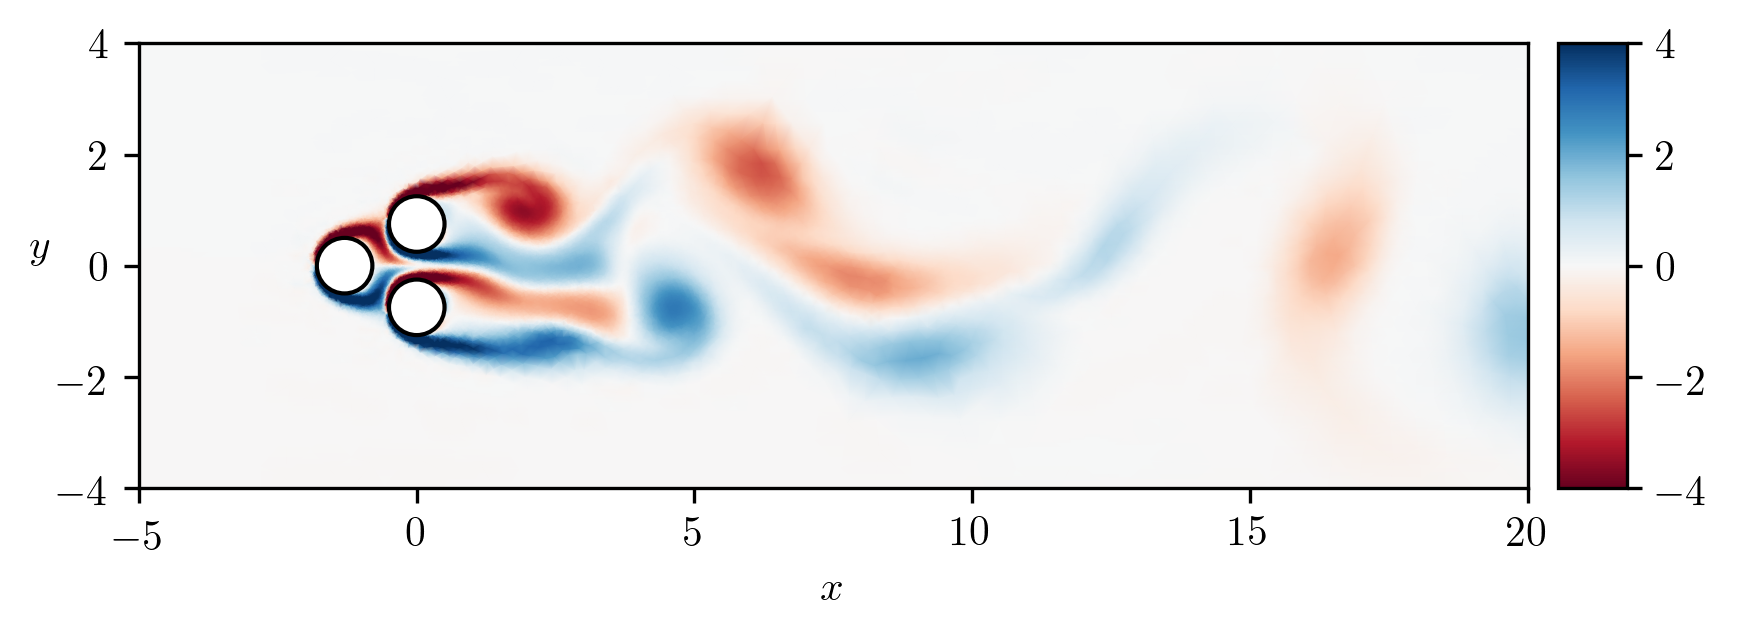
\includegraphics[width=\textwidth]{pinball_dynamics_Re150}}{imgs/pinball_dynamics_Re150.mp4}

			$Re = 150$
	\end{minipage}

	\vspace{1cm}
\end{frame}
%
% \begin{frame}[t, c]{Fluidic Pinball}{Overview of the dynamics}
% 	\centering
% 	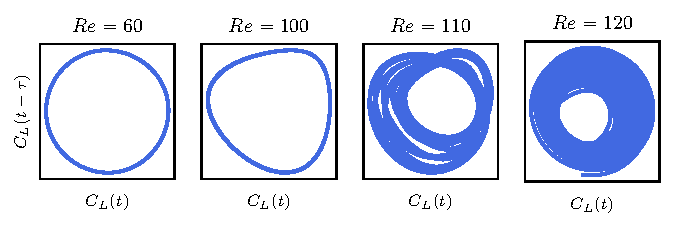
\includegraphics[width=.75\textwidth]{pinball_phase_plots}
%
% 	Low-dimensional phase portraits of the Fluidic pinball's dynamics for $60 \leq Re \leq 120$.
%
% 	\vspace{1cm}
% \end{frame}

\begin{frame}[t, c]{Fluidic Pinball}{\underline{Project}: Investigation of a high-dimensional nonlinear dynamical system}
	\begin{block}{\centering \textbf{Objectives}}
		\centering
		Use the concepts seen during the course to characterize the bifurcations experienced by the flow.
	\end{block}

	\bigskip

	\begin{itemize}
		\item Useful tools/concepts you may use:
		\begin{itemize}
			\item[$\hookrightarrow$] Dimensionality reduction (POD, DMD, ...).
			\item[$\hookrightarrow$] Nonlinear time-series analysis (Lorenz return map, Fourier analysis, Phase portraits, ...)
			\item[$\hookrightarrow$] Reduced-order modeling (Galerkin projection, DMD, System Identification, ...)
		\end{itemize}
	\end{itemize}

	\vspace{1.5cm}
\end{frame}

\begin{frame}[t, c]{Fluidic Pinball}{\underline{Illustration}: Dimensionality reduction}
	\centering
	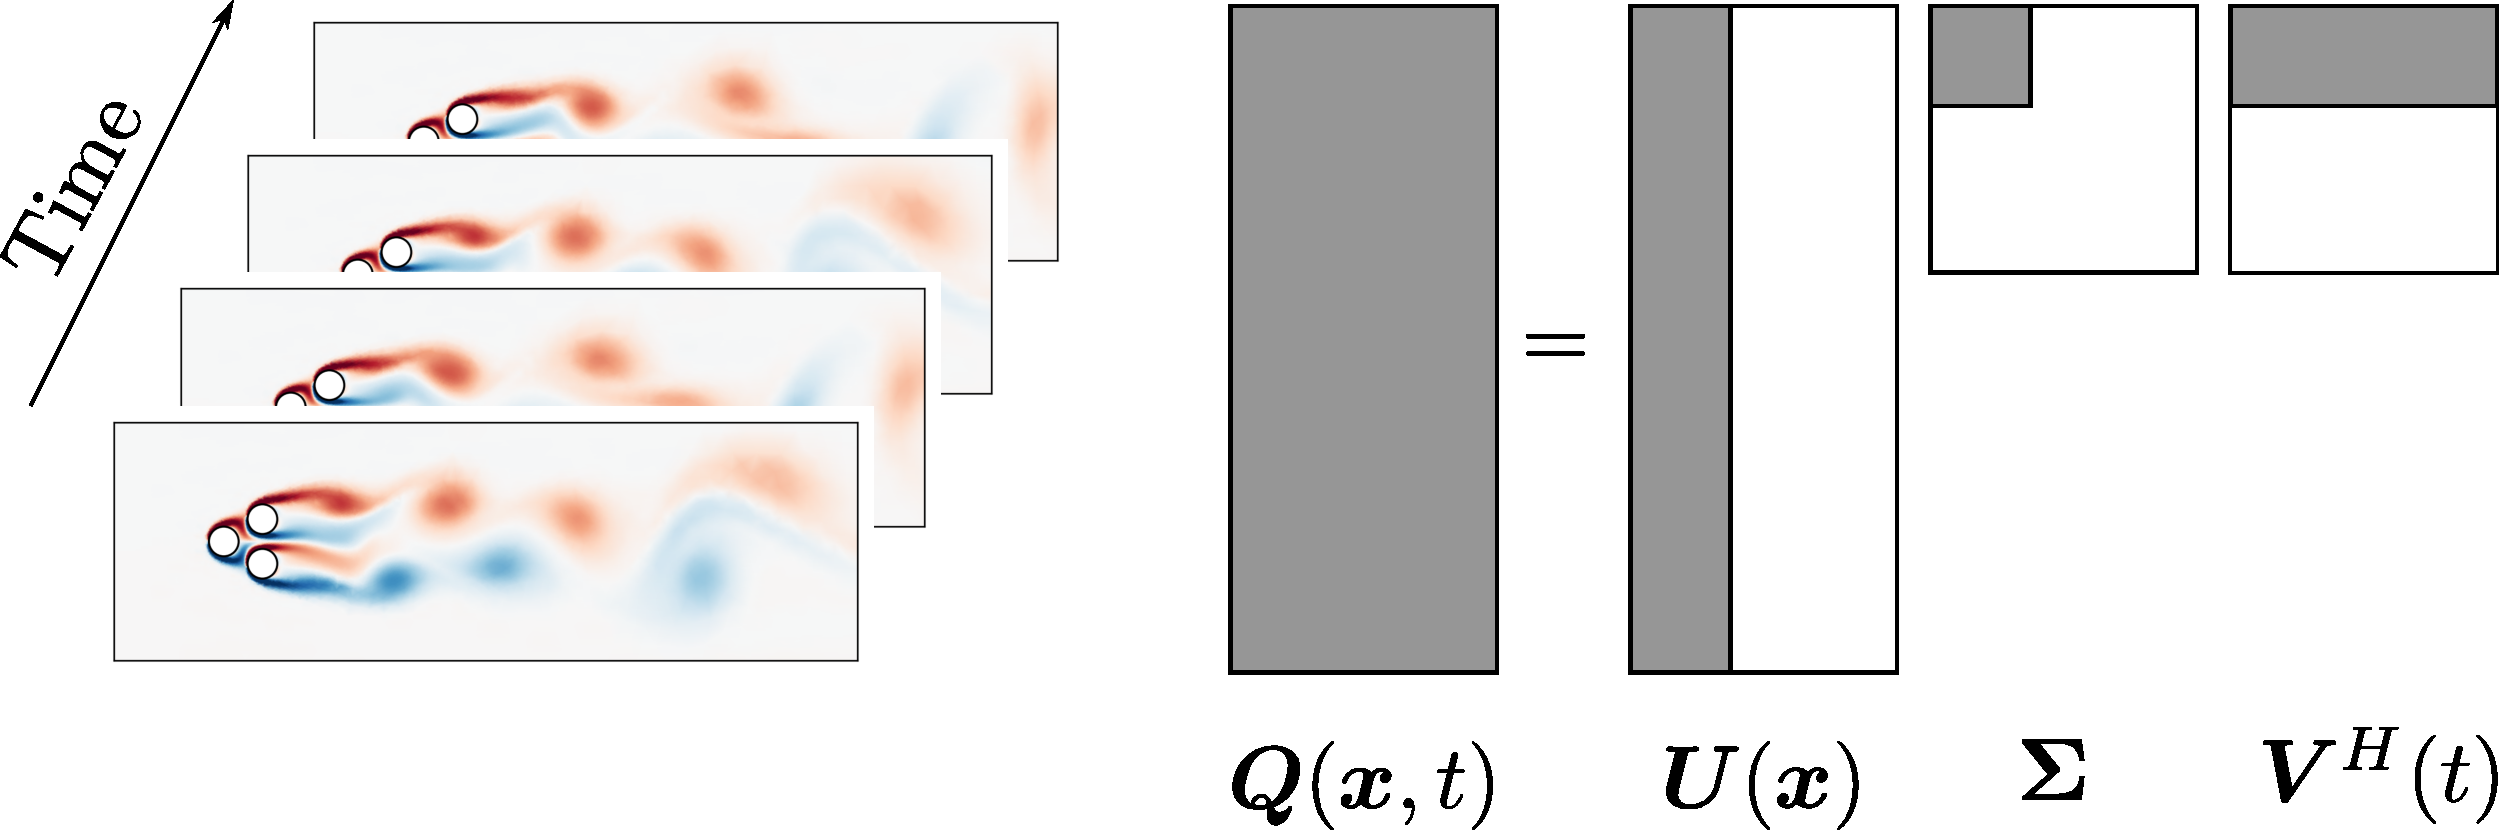
\includegraphics[width=.8\textwidth]{dimensionality_reduction_pinball}

	\bigskip

	Schematic representation of Proper Orthogonal Decomposition.
	\vspace{1cm}
\end{frame}

\begin{frame}[t, c]{Fluidic Pinball}{\underline{Illustration}: Dimensionality reduction}
	\begin{minipage}{.48\textwidth}
		\begin{itemize}
			\item POD/DMD extract \emph{coherent structures} from the data.
			\bigskip
			\item Low-dimensional representation of the system's dynamics.
			\bigskip
			\item Provide a better understanding of the system (e.g.\ reduced-order model).
		\end{itemize}
	\end{minipage}%
	\hfill
	\begin{minipage}{.48\textwidth}
		\centering
		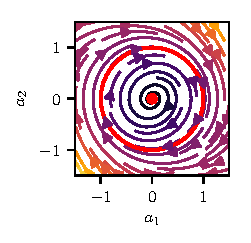
\includegraphics[width=.8\textwidth]{pinball_phase_plane}
	\end{minipage}

	\vspace{1cm}
\end{frame}

\begin{frame}[t, c]{Fluidic Pinball}{Online resources}
	  \begin{minipage}{.9\textwidth}
			\begin{columns}
				\begin{column}{.2\textwidth}
					\centering
					
\includegraphics[height=.15\textheight]{gitlab}
				\end{column}
				\begin{column}{.7\textwidth}
					\url{https://gitlab.com/PinBall/PinBall-A_Toolkit_for_Exploring_MIMO_Flow_Control}
				\end{column}
			\end{columns}
		\end{minipage}
\end{frame}

%-------------------------------------------------------------------------------
%                           KURAMOTO-SHIVASHINSKY
%-------------------------------------------------------------------------------


\begin{frame}[t, c]{}
	\centering
	\vspace{1cm}

	{\Large \textbf{Kuramoto-Sivashinsky}}

	\bigskip

	{\textgre{\textbf{Ring of fire}}}

\end{frame}

\begin{frame}[t, c]{Kuramoto-Sivashinsky}{Ring of fire}
	\begin{itemize}
		\item The Kuramoto-Sivashinsky equation reads
		$$\displaystyle \frac{\partial u}{\partial t} + u \frac{\partial u}{\partial x} = - \frac{\partial^2 u}{\partial x^2} - \frac{\partial^4 u}{\partial x^4},$$
		along with periodic boundary conditions.

		\bigskip

		\item It is a 1D nonlinear PDE describing extended physical systems driven far from equilibrium, instabilities in laminar flame fronts, ...

		\bigskip

		\item Depending on the size $L$ of the computational domain, it can exhibit \alert{\textbf{spatio-temporal chaos}}.
	\end{itemize}

	\vspace{1cm}
\end{frame}

\begin{frame}[t, c]{Kuramoto-Sivashinsky}{Spatio-temporal chaos}
	\centering
	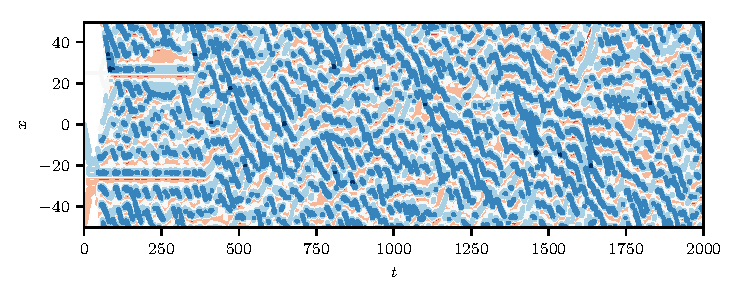
\includegraphics[width=.75\textwidth]{kuramoto_sivashinsky_spatio_temporal_chaos}

	Spatio-temporal dynamics of the Kuramoto-Sivashinsky system for $L = 32 \pi$.

	\vspace{1cm}
\end{frame}

\begin{frame}[t, c]{Kuramoto-Sivashinsky}{\underline{Project}: Instabilities and chaos in a spatially extended system}

	\begin{block}{\centering \textbf{Objectives}}
		\centering
		Combine theoretical and numerical analyses to understand spatio-temporal chaos.
	\end{block}

	\bigskip

	\begin{itemize}
		\item Useful tools/concepts you may use:
		\begin{itemize}
			\item[$\hookrightarrow$] Equilibria and linear stability analysis (Newton, Eigenvalues, ...).
			\item[$\hookrightarrow$] Super- and subcritical bifurcation analysis.
			\item[$\hookrightarrow$] Coherent structures (Fourier modes, POD, DMD, ...)
			\item[$\hookrightarrow$] Nonlinear time-series analysis (Lorenz return map, Fourier analysis, Phase portraits, ...)
		\end{itemize}
	\end{itemize}

	\vspace{1cm}
\end{frame}

\begin{frame}[t, c]{Kuramoto-Sivashinsky}{\underline{Illustration}: Influence of the domain size $L$}
	\centering
	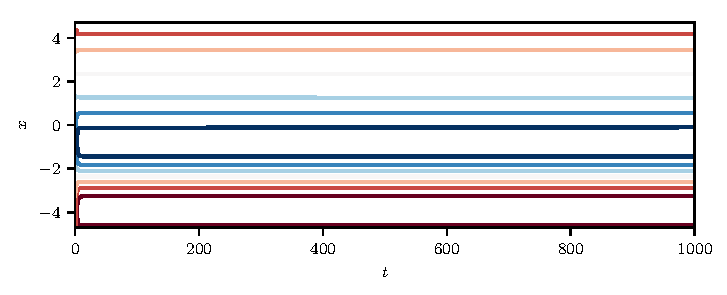
\includegraphics[width=.75\textwidth]{kuramoto_sivashinsky_small_domain}

	Spatio-temporal dynamics of the Kuramoto-Sivashinsky system for $L = 3 \pi$.

	\vspace{1cm}
\end{frame}

\begin{frame}[t, c]{Kuramoto-Sivashinsky}{\underline{Illustration}: Influence of the domain size $L$}
	\centering
	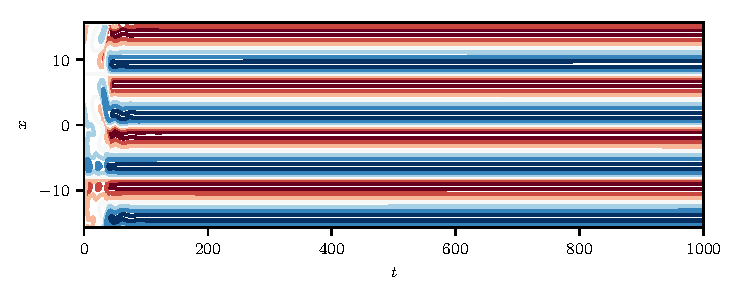
\includegraphics[width=.75\textwidth]{kuramoto_sivashinsky_medium_domain}

	Spatio-temporal dynamics of the Kuramoto-Sivashinsky system for $L = 10 \pi$.

	\vspace{1cm}
\end{frame}

\begin{frame}[t, c]{Kuramoto-Sivashinsky}{\underline{Illustration}: Influence of the domain size $L$}
	\centering
	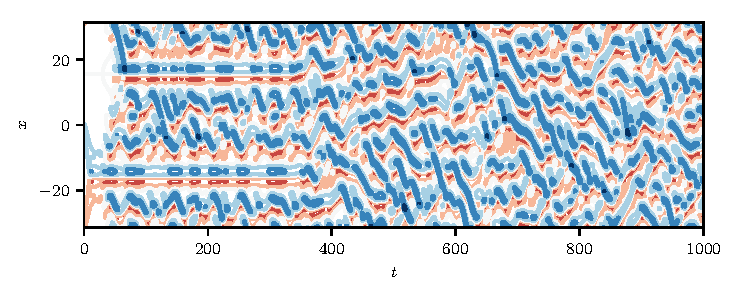
\includegraphics[width=.75\textwidth]{kuramoto_sivashinsky_medium_large_domain}

	Spatio-temporal dynamics of the Kuramoto-Sivashinsky system for $L = 20 \pi$.

	\vspace{1cm}
\end{frame}

\begin{frame}[t, c]{Kuramoto-Sivashinsky}{\underline{Illustration}: Influence of the domain size $L$}
	\centering
	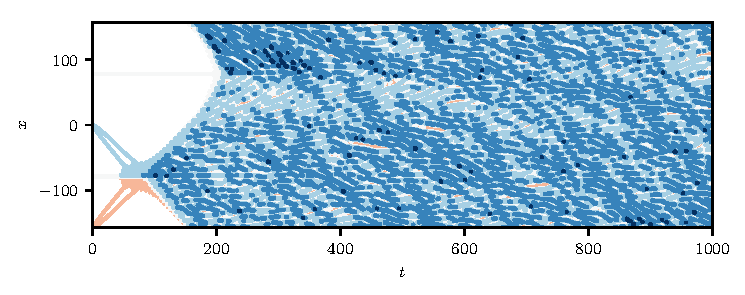
\includegraphics[width=.75\textwidth]{kuramoto_sivashinsky_large_domain}

	Spatio-temporal dynamics of the Kuramoto-Sivashinsky system for $L = 100 \pi$.

	\vspace{1cm}
\end{frame}

\begin{frame}[t, c]{Kuramoto-Sivashinsky}{Online resources}
	  \begin{minipage}{.9\textwidth}
			\begin{columns}
				\begin{column}{.2\textwidth}
					\centering
					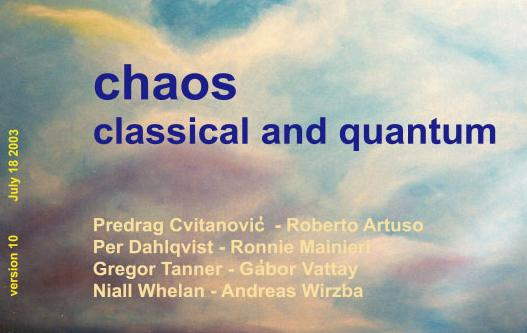
\includegraphics[height=.15\textheight]{chaosbook}
				\end{column}
				\begin{column}{.7\textwidth}
					\url{http://chaosbook.org/extras/KSEproject/html/index.html}
				\end{column}
			\end{columns}
		\end{minipage}
\end{frame}


%-------------------------------------------------------------------------------
%                           CELLULAR AUTOMATON
%-------------------------------------------------------------------------------


\begin{frame}[t, c]{}
	\centering
	\vspace{1cm}

	{\Large \textbf{Agent-based models}}

	\bigskip

	{\textgre{\textbf{A discrete universe}}}

\end{frame}

\begin{frame}[t, c]{Agent-based models}{Discrete universe}
	\begin{minipage}{.48\textwidth}
		\begin{itemize}
			\item Discrete time, discrete space and discrete state model studied in a wide range of domains.

			\bigskip

			\item Evolution is guided by very simple rules.

			\bigskip

			\item One of the most famous is \alert{\textbf{Conway's Game of Life}} (cellular automaton).
		\end{itemize}
	\end{minipage}%
	\hfill
	\begin{minipage}{.48\textwidth}

	\end{minipage}

	\vspace{1cm}
\end{frame}

\begin{frame}[t, c]{Predator-Prey interactions}{\underline{Project}: Two different models for predator-prey interactions}

		\begin{block}{\centering \textbf{Objectives}}
			\centering
			Use discrete-time dynamical systems to model predator-prey interactions observed in "real life".
		\end{block}

		\bigskip

		\begin{itemize}
			\item Useful tools/concepts you may use:
			\begin{itemize}
				\item[$\hookrightarrow$] Equilibria and linear stability analysis of discrete-time systems.
				\item[$\hookrightarrow$] System identification (NARMAX).
				\item[$\hookrightarrow$] Nonlinear time-series analysis (Fourier analysis, Phase portraits, ...).
			\end{itemize}
		\end{itemize}

		\vspace{1cm}
\end{frame}

% \begin{frame}[t, c]{Predator-Prey interactions}{\underline{Illustration}: Agent-based model}
%
% \end{frame}

\begin{frame}[t, c]{Predator-Prey interactions}{\underline{Illustration}: Discrete-time dynamical system}
	\begin{minipage}{.48\textwidth}
		\begin{itemize}
			\item These dynamics can be modeled by
			\begin{equation}
				\begin{aligned}
					x_{k+1} & = a x_k ( 1 - x_k ) - b x_k y_k \\
					y_{k+1} & = c y_k + d x_k y_k,
				\end{aligned}
				\notag
			\end{equation}
			where $x_k$ and $y_k$ are the prey and predator's population, respectively.

			\bigskip

			\item Parameters $a$, $b$, $c$ and $d$ can be estimated using "real life" observations.
		\end{itemize}
	\end{minipage}%
	\hfill
	\begin{minipage}{.48\textwidth}
		\centering
		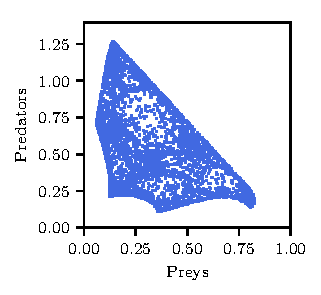
\includegraphics[width=.8\textwidth]{lotka_volterra}
	\end{minipage}

	\vspace{1cm}
\end{frame}

\begin{frame}[t, c]{Predator-Prey interactions}{Online resources}
	  \begin{minipage}{.9\textwidth}
			\begin{columns}
				\begin{column}{.2\textwidth}
					\centering
					
\includegraphics[height=.15\textheight]{gitlab}
				\end{column}
				\begin{column}{.7\textwidth}
					\url{https://gitlab.com/PinBall/PinBall-A_Toolkit_for_Exploring_MIMO_Flow_Control}
				\end{column}
			\end{columns}
		\end{minipage}
\end{frame}

\end{document}
